% Sections 3.5 (red-line classification) and 3.6 (other remnant diagnostics) of the Silk Nebula comment
\subsection{Red-line ratios do not classify the \texorpdfstring{\Oiii{}}{[O III]} filament}\label{sec:shock}

W26 Sect.~4.1 classifies the ionized gas as shock-excited from red-line criteria that separate remnants from \ion{H}{2} regions \citep{Fesen1985}: \Sii~$\lambda\lambda$6716,\,6731/\Ha{} ``exceeds 0.5 in all four regions'', \Nii/\Ha{} lies within 0.5--1.5, and the points fall in the remnant zones of the \citet{Sabin2013} and \citet{Kopsacheili2020} diagrams (W26 Fig.~8, whose three panels use only \Ha, \Nii{} and \Sii). The \Sii/\Ha{} threshold varies within W26 between 0.4 and 0.5.

These ratios do not distinguish the filament from its surroundings. The W26 Table~2 intensities give \Sii/\Ha{} $=0.90\pm0.11$, $0.86\pm0.09$ and $0.81\pm0.13$ in P1--P3 and $0.80\pm0.13$ in the nebula-free region P4, and \Nii~$\lambda$6583/\Ha{} $=0.80$, 0.70 and 0.77 ($\pm0.09$--0.10) against $0.80\pm0.10$ (Figure~\ref{fig:redline}a); no filament region differs from P4 by more than $0.72\sigma$. P4 therefore meets the W26 criteria too, as W26 Sects.~4.1 and~4.2 note, and in all three panels of W26 Fig.~8 the background points overlap the filament points; W26 nevertheless concludes that the remnant dominates and the diffuse-gas contribution is minor.

The values are those of the faint high-latitude WIM. \citet{Madsen2006} find \Sii~$\lambda$6716/\Ha{} $\gtrsim0.4$ where \Ha{} is faint ($\gtrsim0.68$ for the doublet sum at the low-density limit) and \Nii/\Ha{} $\gtrsim0.7$ in the faintest WIM at $\ell>150\arcdeg$, against means of 0.11 and 0.27 in O-star \ion{H}{2} regions; both ratios rise as \Ha{} fades, which they and \citet{Haffner1999} attribute to WIM temperature variations. Toward P1--P4 the nearest WHAM beams \citep{Haffner2003} give 2.9--4.4\,R of \Ha, and neither WHAM (on$-$off $\Delta I=+0.04\pm0.35$\,R in the south) nor the SDSS sky fibers ($0.08\pm0.22$\,R at Dec $<17.6\arcdeg$) shows an excess on the filament.

The MRS-N red lines therefore trace foreground and background WIM, consistent with the diffuse-ionized-gas contribution inferred in W26 Sect.~4.2; thresholds that separate remnants from \ion{H}{2} regions do not separate them from the WIM at a few rayleighs. With no \Hb{} in the blue arm and no red-line ratio that isolates the \Oiii-emitting gas, the MRS-N data do not constrain the excitation of the filament. This is not evidence against shock excitation, which Section~\ref{sec:excitation} tests with \Oiii/\Hb{} and other diagnostics.

\begin{figure*}
\centering
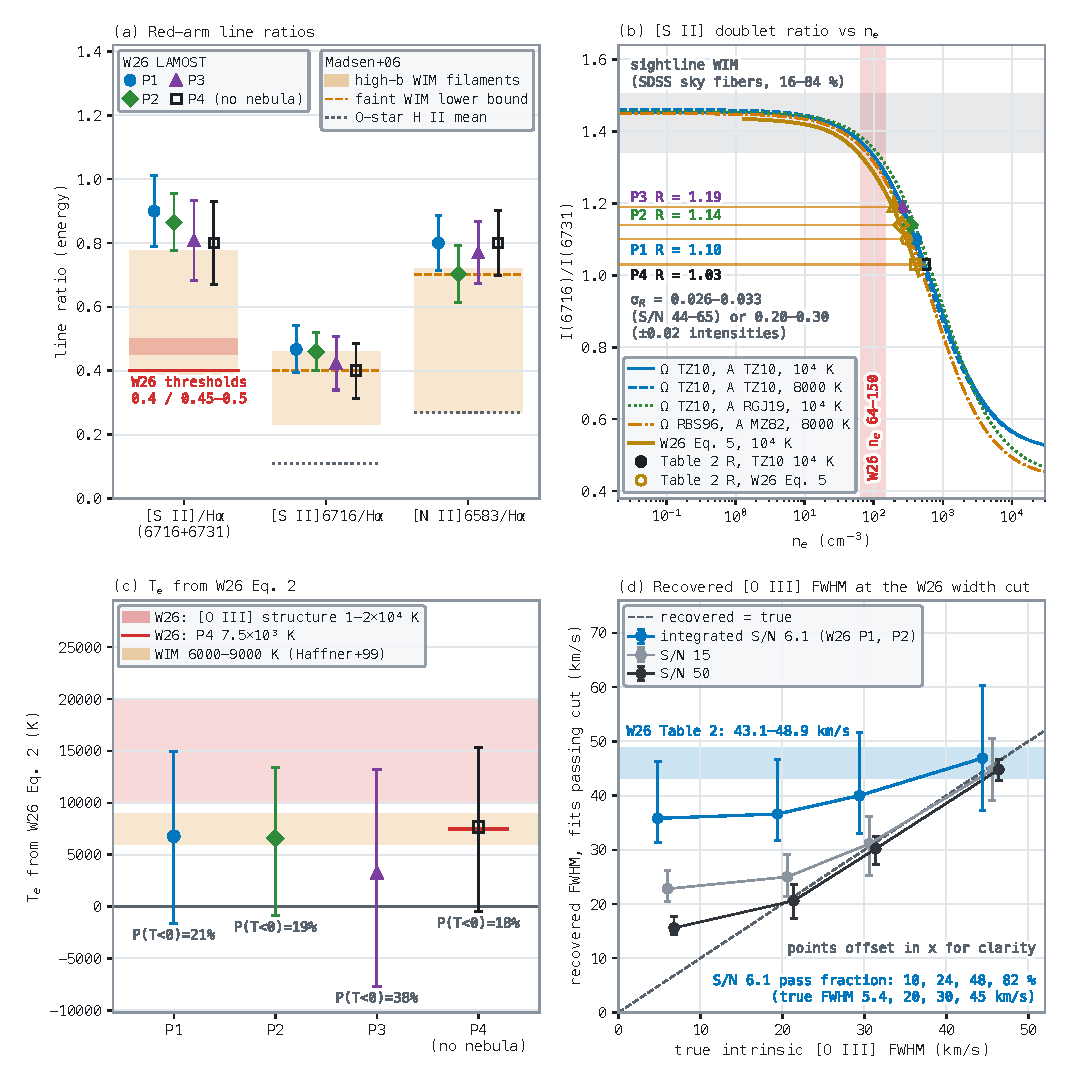
\includegraphics[width=\textwidth]{figures/dispute_other_fig6.pdf}
\caption{Tests of the W26 \citep{Wu2026} diagnostics with W26 Table~2 values (P1--P3, filament; P4, nebula-free). (a) Red-arm line ratios (energy units; $1\sigma$ errors) with the warm-ionized-medium (WIM) and \ion{H}{2}-region values of \citet{Madsen2006}; the shading for the doublet sum assumes the low-density limit. (b) $I(6716)/I(6731)$ versus electron density $n_e$ for a five-level S$^+$ atom (collision strengths $\Omega$ and transition probabilities $A$ from TZ10, \citealt{Tayal2010}; RBS96, \citealt{Ramsbottom1996}; MZ82, \citealt{Mendoza1982}; RGJ19, \citealt{Rynkun2019}) and for W26 Eq.~5 \citep{Proxauf2014}; markers, W26 Table~2 ratios; gray band, WIM in SDSS sky fibers \citep{Abdurrouf2022,SDSS2026}. (c) $T_e$ from W26 Eq.~2 (Monte Carlo 16th--84th percentiles) and $P(T<0)$; WIM range from \citet{Haffner1999}. (d) Recovered versus true \Oiii{} FWHM (median, 16th--84th percentiles) of simulated fits passing the W26 width cut, by integrated S/N.}
\label{fig:redline}
\end{figure*}

\subsection{Other remnant diagnostics}\label{sec:snrdiag}

\textit{Electron density.} W26 derives a mean $n_e\approx64$\,cm$^{-3}$ from 107 per-fiber values (W26 Fig.~7b), rising to $\approx150$\,cm$^{-3}$ toward the center, from the \Sii{} doublet with its Eq.~5 \citep{Proxauf2014} and assigns it to the \Oiii-emitting gas (W26 Sects.~3.4, 4.1). The regional W26 Table~2 ratios, $R=I(6716)/I(6731)=1.03$--1.19, give 169--400\,cm$^{-3}$ with W26 Eq.~5 and 225--631\,cm$^{-3}$ with a five-level S$^+$ atom at 8000--$10^4$\,K \citep{Tayal2010,Ramsbottom1996,Mendoza1982,Rynkun2019}. They lie 5.6--9.2$\sigma$ below the $R=1.33$ that W26 Eq.~5 requires for 64\,cm$^{-3}$ if $\sigma_R=0.026$--0.033 (W26 Table~2 S/N), and constrain no density if $\sigma_R=0.20$--0.30 (independent $\pm0.02$ intensity errors; Figure~\ref{fig:redline}b). Either way, the doublet traces the WIM, which SDSS sky fibers and DESI place at the low-density limit on this sightline ($R=1.40$; 1.34--1.50 and 1.33--1.49). The \Oiii{} gas needs only $n_e\approx0.1$--3\,cm$^{-3}$ to emit 2--4\,R (measured: 1.4--2.5\,R; Section~\ref{sec:brightness}) at $\approx$280\,pc (Section~\ref{sec:location}).

\textit{Temperature and turbulence.} W26 Eq.~2 \citep{Reynolds1977} and W26 Table~2 \Ha{} and \Nii{} widths give $T=6780$, 6580, 3220 and 7660\,K for P1--P4, with $\sigma_T=7300$--10700\,K and $P(T<0)=18$--38\% (Figure~\ref{fig:redline}c), so the regional widths do not show P1--P3 to be hotter than P4, as W26 Sect.~3.4 reports from per-fiber values (1--2$\times10^4$\,K on the structure, $7.5\times10^3$\,K in P4). W26 Eq.~3 gives $V_t=25.7$--29.9\,\kms{} for P1--P3 and 26.5\,\kms{} for P4 (W26 Table~4: 30.6--33.1 and 29.9\,\kms); P4 again matches P1--P3, as expected for WIM broadening.

\textit{Abundances.} The N2 index, $\log$(\Nii~$\lambda$6583/\Ha) $=-0.153$ to $-0.097$, lies outside the calibrated range of W26 Eq.~6 \citep[$-2.5<{\rm N2}<-0.3$;][]{Pettini2004}. P1--P3 give $12+\log({\rm O/H})=8.81$--8.84 with W26 Eq.~6 and 8.64--8.72 with N2S2H$\alpha$ \citep{Dopita2016}; P4 gives 8.84 and 8.75. Both calibrations assume stellar photoionization, whereas in the WIM a high \Nii/\Ha{} traces a higher electron temperature, not a higher N/H \citep{Haffner1999,Madsen2006}; the derived O/H describes the WIM.

\textit{\Oiii{} line width.} The intrinsic \Oiii{} widths in W26 Table~2 (FWHM 43.1--48.9\,\kms) do not distinguish an unresolved line from a 45\,\kms{} one: simulated fits that pass the acceptance cut of W26 Sect.~3.2.2 (assumed blue-arm instrumental FWHM $40\pm1.5$\,\kms) at S/N 6.1 (W26 Table~2), taken as integrated, return median FWHM of 35.8--46.9\,\kms{} for true FWHM of 5.4--45\,\kms{} (Figure~\ref{fig:redline}d). W26 does not define its S/N; for a peak S/N the bias is smaller and the widths would indicate $\approx45$\,\kms.

\textit{Energetics.} The W26 inputs reproduce the shock velocity $v_s=119.3$\,\kms{} \citep{Dopita1979}, the explosion energy $E=2.01\times10^{51}$\,erg \citep{Boumis2022} and, within the quoted uncertainties, the radius at the onset of the pressure-driven snowplow (PDS) phase ($R_{\rm PDS}=17.1$\,pc against $18\pm2.8$\,pc) and the age ($7.95\times10^4$\,yr against $(6.8\pm1.8)\times10^4$\,yr; \citealt{Cioffi1988}); the ``$+1$'' in the printed age formula, where \citet{Cioffi1988} has ``$+1/3$'', is a misprint that does not affect the quoted age. The inputs are unsupported: the shell radius $R_s=30$\,pc follows from the 160\,pc distance (Section~\ref{sec:distance}), the ambient density $n_0=1.0\pm0.3$\,cm$^{-3}$ is adopted, and $v_s$ derives from the WIM \Sii{} density. A complete radiative shock emits at least 0.117 \Hb{} photons per swept-up H atom, so the \Hb{} non-detection in the spectra of Section~\ref{sec:spectrum} ($I({\rm H}\beta)\le0.15$\,R at $2\sigma$, from \Oiii/\Hb{} $>11$ at 1.62\,R in DESI), with limb brightening of 3--18.6, bounds such a shock at $\approx$280\,pc to $n_0\le0.005$--0.043\,cm$^{-3}$ and $E\le4.2\times10^{49}$--$3.8\times10^{50}$\,erg (model scalings); incomplete shocks (Section~\ref{sec:excitation}) are exempt.

\textit{Radio.} W26 Sect.~4.1 takes the absence of counterparts in the NRAO VLA Sky Survey (NVSS; \citealt{Condon1998}) and the TIFR GMRT Sky Survey (TGSS; \citealt{Intema2017}) as consistent with an old remnant. These interferometric surveys resolve out smooth structure wider than $\approx8\arcmin$ \citep[NVSS snapshots;][]{NRAO2025} and 10\arcmin--20\arcmin{} \citep[TGSS;][]{Intema2017}; the filament is 17\arcmin{} wide, so the non-detection is uninformative.
